\section*{CHƯƠNG 2. TỔNG QUAN LÝ THUYẾT VÀ CÔNG NGHỆ}
    \addcontentsline{toc}{section}{\numberline{} CHƯƠNG 2. TỔNG QUAN LÝ THUYẾT VÀ CÔNG NGHỆ}

\setcounter{section}{2}
    \setcounter{subsection}{0}
        \setcounter{figure}{0}
            \setcounter{table}{0}
%---------------------------------------------------------%

\subsection{Tổng quan về chủ đề nghiên cứu}

\subsubsection{Lịch sử phát triển cột bơm xăng dầu \cite{first-gas-pump-and-service-station}} 

Cột bơm xăng dầu (fuel dispenser hay gas pump) là thiết bị thiết yếu trong hệ thống trạm nhiên liệu, được sử dụng để bơm nhiên liệu như xăng hoặc dầu diesel vào phương tiện giao thông. Trong suốt hơn một thế kỷ qua, thiết bị này đã trải qua nhiều giai đoạn cải tiến về mặt cơ khí, điện tử và an toàn.

Cột bơm đầu tiên được phát minh vào năm 1885 bởi Sylvanus Bowser tại Fort Wayne, Indiana (Hoa Kỳ), ban đầu được thiết kế để bơm kerosene cho mục đích thắp sáng và nấu ăn. Sau đó, khi ô tô trở nên phổ biến vào đầu thế kỷ 20, thiết kế này nhanh chóng được cải tiến để phục vụ việc phân phối xăng.

Đến năm 1905, công ty Bowser đã giới thiệu dòng sản phẩm \textit{Self-Measuring Gasoline Storage Pump} - thiết bị đầu tiên kết hợp bộ đo thể tích nhiên liệu, giúp người dùng biết được chính xác lượng nhiên liệu được bơm. Các phiên bản ban đầu có cấu trúc thủ công, sử dụng tay quay để bơm nhiên liệu, và có bình thủy tinh trong suốt phía trên nhằm đo thể tích bằng mắt thường.

Vào những năm 1920-1930, các công ty như Tokheim, Wayne và Gilbarco đã bắt đầu phát triển các trạm bơm hiện đại hơn, với bơm điện thay thế hệ thống tay quay. Bên cạnh đó, thiết kế cột bơm cũng bắt đầu được cải tiến để đảm bảo an toàn, chẳng hạn như sử dụng van ngắt tự động và ống bơm linh hoạt hơn nhằm tránh cháy nổ.

Sau Thế chiến II, đặc biệt từ những năm 1950 trở đi, cột bơm chuyển dần sang dạng thiết bị tự động hoá, có tích hợp đồng hồ đo cơ học, công tơ mét và bảng hiển thị giá thành. Ngày nay, công nghệ vi xử lý được tích hợp, cho phép cột bơm giao tiếp với hệ thống thanh toán, quản lý tồn kho và giám sát từ xa.

Ngày nay, các cột bơm xăng dầu hiện đại không chỉ đảm bảo độ chính xác trong việc đo lường và phân phối nhiên liệu, mà còn được tích hợp các tính năng kỹ thuật số như: màn hình cảm ứng, thanh toán không tiếp xúc (contactless), nhận diện phương tiện tự động, kết nối internet để cập nhật giá xăng theo thời gian thực và thậm chí cung cấp quảng cáo trực tiếp trên màn hình bơm.

\begin{figure}[!ht]
    \centering
    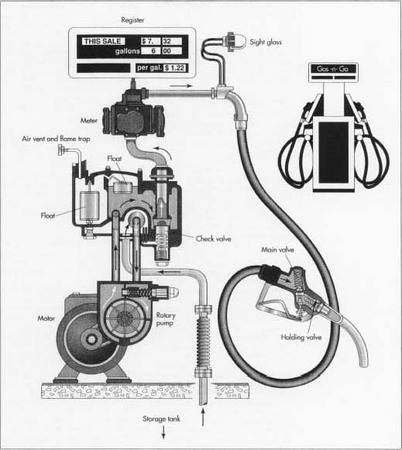
\includegraphics[width=0.6\linewidth]{Figures/Chap2_typical-gas-pump-mechanism.jpg}
    \caption{Nguyên lý hoạt động các cột bơm xăng dầu phổ biến}
    \label{fig:Chap2_typical-gas-pump-mechanism}
\end{figure}
\FloatBarrier

Sự phát triển của cột bơm xăng dầu phản ánh sự tiến bộ chung của ngành giao thông và công nghệ nhiên liệu, với mục tiêu cuối cùng là tối ưu hóa hiệu quả, an toàn và trải nghiệm người dùng.


\subsubsection{Màn hình cột bơm xăng dầu}

Màn hình cột bơm xăng dầu hiển thị các thống số sau:

\begin{itemize}
    \item \textbf{Tổng}: Tổng số tiền ứng với số lít lượng xăng/dầu đã bơm.
    \item \textbf{Lít}: Số lít xăng/dầu đã bơm.
    \item \textbf{Đơn giá}: Số tiền trên một lít xăng/dầu
\end{itemize}

Màn hình sẽ có 3 hàng hiển thị giá trị tương ứng với cho 3 thông số trên.

Đối với hầu hết các loại cột bơm xăng dầu cũ, phổ biến trên thị trường hiện tại nói chung và với cột bơm hãng ZCheng - là đối tượng nghiên cứu của đồ án - nói riêng, màn hình cột bơm gồm 3 hàng hiển thị bằng các LED 7 thanh (hình \ref{fig:Zcheng-screen}). IC màn hình sẽ nhận dữ liệu từ bầu lường, sau đó điều khiển hiển thị từng LED.

\begin{figure}[!ht]
    \centering
    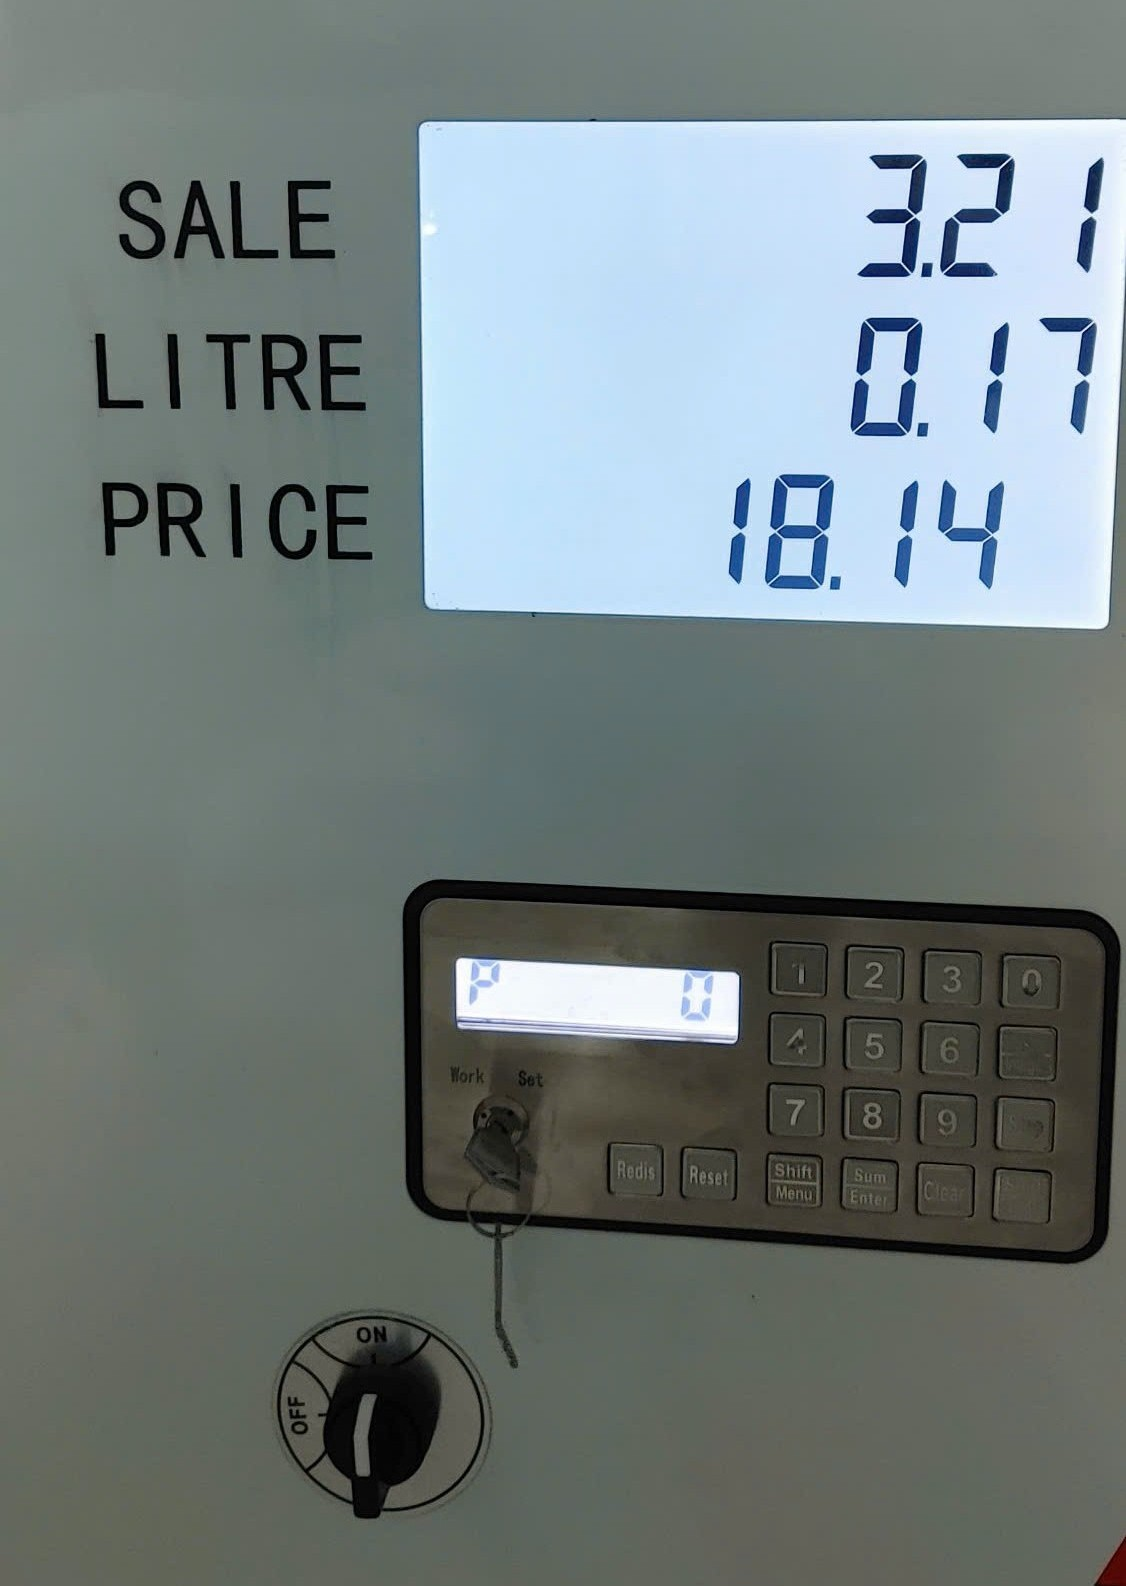
\includegraphics[width=0.45\linewidth]{Figures/ZCheng_gas-pump-screen.jpg}
 
    \caption{Màn hình hiển thị cột bơm ZCheng sử dụng các LED 7 thanh}
    \label{fig:Zcheng-screen}
\end{figure}

\FloatBarrier

\subsection{Cơ sở lý thuyết}

\subsubsection{LED 7 thanh} 

LED 7 thanh\cite{luong2020dientuso} (Seven-segment display) là một loại linh kiện hiển thị phổ biến dùng để hiển thị các chữ số thập phân (0–9) và một số ký tự chữ cái nhất định. Thiết bị này bao gồm 7 đoạn LED riêng biệt (ký hiệu là a, b, c, d, e, f, g), được sắp xếp theo hình dạng số 8. Mỗi đoạn là một LED nhỏ có thể phát sáng riêng biệt, cho phép tổ hợp thành các chữ số bằng cách điều khiển bật/tắt từng đoạn.



\begin{figure}[!ht]
    \centering
    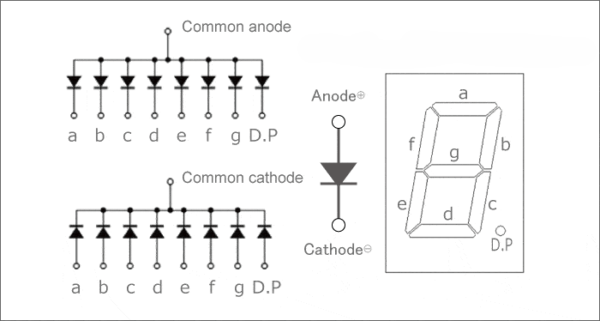
\includegraphics[width=0.8\linewidth]{Figures/Chap2_7-seg-led.png}
    \caption{Cấu trúc của LED 7 thanh}
     \label{fig:Chap2_7-seg-led}
\end{figure}

\textbf{Phân loại:}
\begin{itemize}
    \item \textbf{Anode chung (Common Anode):} tất cả các cực dương (anode) của các LED được nối chung với nhau. Để bật một đoạn LED, ta cấp mức thấp (LOW) vào chân tương ứng.
    \item \textbf{Cathode chung (Common Cathode):} tất cả các cực âm (cathode) của các LED được nối chung với nhau. Để bật một đoạn LED, ta cấp mức cao (HIGH) vào chân tương ứng.
\end{itemize}

\textbf{Bảng mã hiển thị:}

\begin{table}[H]
    \centering
    \caption{Bảng mã nhị phân điều khiển LED 7 thanh hiển thị chữ số (Common Cathode)}
    \begin{tabular}{|c|c|}
        % \hline
        Chữ số & Các đoạn sáng (abcdefg) \\
        \hline
        0 & 1111110 \\
        1 & 0110000 \\
        2 & 1101101 \\
        3 & 1111001 \\
        4 & 0110011 \\
        5 & 1011011 \\
        6 & 1011111 \\
        7 & 1110000 \\
        8 & 1111111 \\
        9 & 1111011 \\
        \hline
    \end{tabular}
\end{table}

\textbf{Ứng dụng:} LED 7 thanh thường được sử dụng trong các thiết bị hiển thị đơn giản như đồng hồ điện tử, màn hình cột bơm xăng dầu, bộ đếm số, máy tính bỏ túi, mạch đo số, và các hệ thống nhúng cần hiển thị dữ liệu dạng số.

Việc điều khiển LED 7 thanh có thể thực hiện thông qua vi điều khiển bằng cách xuất tín hiệu logic ra từng chân tương ứng. Ngoài ra, có thể sử dụng IC giải mã như 74LS47 hoặc 74HC595 để giảm số chân điều khiển và đơn giản hóa mạch.


\subsubsection{Giao thức SPI }

Giao thức \textbf{SPI\cite{st_rm_f4} (Serial Peripheral Interface) } là một giao thức truyền thông nối tiếp đồng bộ do hãng Motorola đề xuất vào cuối thập niên 1980. SPI cho phép truyền dữ liệu tốc độ cao giữa vi điều khiển và các thiết bị ngoại vi như cảm biến, bộ nhớ Flash, DAC, ADC, màn hình LCD, v.v.

\textbf{1. Kiến trúc tổng quát}

SPI là giao thức theo mô hình \textbf{Master - Slave}, trong đó một thiết bị Master điều khiển một hoặc nhiều thiết bị Slave. Kết nối SPI sử dụng bốn đường tín hiệu chính:

\begin{itemize}
    \item \textbf{MOSI (Master Out - Slave In)}: Dữ liệu từ Master truyền sang Slave.
    \item \textbf{MISO (Master In - Slave Out)}: Dữ liệu từ Slave truyền về Master.
    \item \textbf{SCLK (Serial Clock)}: Xung nhịp do Master tạo ra để đồng bộ dữ liệu.
    \item \textbf{SS (Slave Select)}: Tín hiệu chọn Slave (còn gọi là CS - Chip Select), khi mức thấp thì thiết bị Slave tương ứng được kích hoạt.
\end{itemize}


\textbf{2. Cơ chế truyền dữ liệu}

SPI hoạt động theo nguyên tắc truyền song song hai chiều (full duplex). Mỗi lần đồng hồ (SCLK) tạo ra một chu kỳ, dữ liệu trên MOSI và MISO đều được dịch chuyển một bit. Cả Master và Slave đều có bộ dịch (shift register), cho phép vừa gửi vừa nhận dữ liệu đồng thời.

\begin{itemize}
    \item Truyền dữ liệu theo từng byte (8 bit) hoặc nhiều byte liên tiếp.
    \item Thứ tự truyền bit có thể là MSB first hoặc LSB first tùy cấu hình.
    \item Tần số xung đồng hồ thường trong khoảng vài trăm kHz đến hàng chục MHz.
\end{itemize}

\textbf{3. Ưu và nhược điểm}

\textbf{Ưu điểm:}
\begin{itemize}
    \item Tốc độ truyền cao (cao hơn I\textsuperscript{2}C).
    \item Truyền dữ liệu song công (full duplex).
    \item Giao thức đơn giản, dễ cài đặt.
\end{itemize}

\textbf{Nhược điểm:}
\begin{itemize}
    \item Không hỗ trợ truyền đa điểm (mỗi Slave cần một chân SS riêng).
    \item Không có cơ chế xác thực hoặc kiểm tra lỗi tích hợp.
    \item Khoảng cách truyền ngắn (thường < 1m).
\end{itemize}

\textbf{4. Ứng dụng}

SPI được sử dụng rộng rãi trong các hệ thống nhúng có yêu cầu tốc độ cao, như:
\begin{itemize}
    \item Giao tiếp với màn hình TFT, OLED.
    \item Đọc/ghi bộ nhớ Flash, EEPROM.
    \item Điều khiển cảm biến tốc độ cao (IMU, ADC,...).
\end{itemize}

SPI là một trong những giao thức truyền thông có dây phổ biến nhất hiện nay trong lĩnh vực điện tử nhúng, nhờ tính đơn giản, tốc độ cao và dễ triển khai.

\FloatBarrier
\subsubsection{Mạng LAN}

\textbf{LAN (Local Area Network)\cite{cloudflare_lan}} là mạng máy tính cục bộ, cho phép nhiều thiết bị trong một khu vực địa lý nhỏ (như một tòa nhà, văn phòng hoặc nhà máy) kết nối và chia sẻ tài nguyên với nhau, chẳng hạn như dữ liệu, thiết bị ngoại vi, hoặc truy cập Internet.

\textbf{1. Kiến trúc cơ bản}

Một mạng LAN thường bao gồm:

\begin{itemize}
    \item \textbf{Các thiết bị đầu cuối (end devices)}: Máy tính, máy chủ, thiết bị nhúng, camera, v.v.
    \item \textbf{Thiết bị mạng (network devices)}: Switch, router, hub, access point,...
    \item \textbf{Phương tiện truyền dẫn (medium)}: Cáp mạng (Ethernet – Cat5e, Cat6) hoặc kết nối không dây (Wi-Fi).
\end{itemize}

\begin{figure}[!ht]
    \centering
    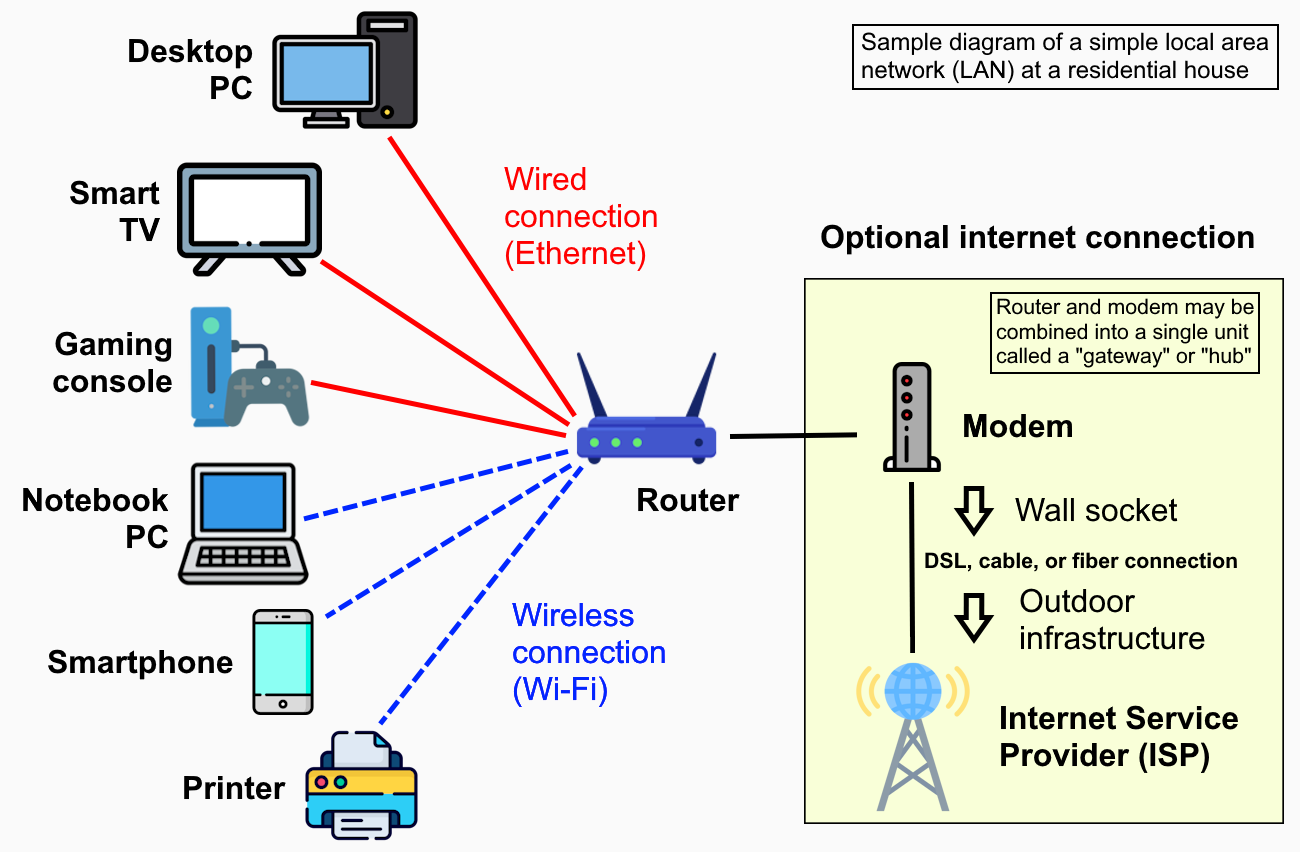
\includegraphics[width=0.8\linewidth]{Figures/Chap2_LAN-network.png}
    \caption{Tổ chức mạng LAN}
     \label{fig:Chap2_LAN-network}
\end{figure}


LAN sử dụng các giao thức truyền thông tầng thấp như Ethernet (IEEE 802.3) và tầng cao như TCP/IP để định tuyến và truyền dữ liệu giữa các thiết bị.

\textbf{2. Ưu điểm của mạng LAN}
\begin{itemize}
    \item Tốc độ truyền dữ liệu cao (10Mbps đến 10Gbps).
    \item Độ trễ thấp, phù hợp với các hệ thống điều khiển thời gian thực.
    \item Dễ dàng mở rộng, bảo trì và quản lý.
    \item Chi phí triển khai thấp trong phạm vi nhỏ.
\end{itemize}

\textbf{3. Ứng dụng trong hệ thống kỹ thuật}
LAN đóng vai trò quan trọng trong các hệ thống kỹ thuật hiện đại:

\begin{itemize}
    \item Giao tiếp giữa thiết bị nhúng và máy chủ điều khiển.
    \item Hệ thống giám sát và điều khiển công nghiệp (SCADA, HMI).
    \item Chia sẻ dữ liệu giữa các cảm biến, bộ điều khiển và thiết bị hiển thị.
\end{itemize}



\textbf{4. Các giao thức phổ biến trong LAN}
LAN hỗ trợ nhiều giao thức như:
\begin{itemize}
    \item \textbf{Ethernet (IEEE 802.3)} – Giao thức truyền thông vật lý và MAC trong hầu hết hệ thống LAN có dây.

    \item \textbf{ARP (Address Resolution Protocol)} – Dùng để ánh xạ địa chỉ IP sang địa chỉ MAC.
    \item \textbf{DHCP (Dynamic Host Configuration Protocol)} – Gán IP động cho các thiết bị trong mạng.
    \item \textbf{TCP/IP} – Giao thức tầng truyền tải và mạng, chịu trách nhiệm truyền dữ liệu tin cậy giữa các thiết bị.
\end{itemize}



Mạng LAN là nền tảng kết nối thiết bị trong hệ thống điện tử hiện đại, giúp các thành phần hoạt động đồng bộ, truyền dữ liệu hiệu quả và dễ dàng mở rộng quy mô hệ thống.

\FloatBarrier

\subsection{Kiến trúc giao thức TCP/IP}

Giao thức TCP/IP\cite{hoang_mangtruyenthongcongnghiep} (Transmission Control Protocol/Internet Protocol) là nền tảng của mạng Internet và hầu hết các mạng máy tính hiện đại. Đây là một bộ giao thức gồm nhiều lớp, được thiết kế để đảm bảo việc truyền dữ liệu giữa các thiết bị trong môi trường mạng không đồng nhất. Kiến trúc TCP/IP được phát triển bởi Bộ Quốc phòng Hoa Kỳ vào những năm 1970 và dần trở thành chuẩn thực tế trong lĩnh vực truyền thông mạng.

\begin{figure}[H]
    \centering
    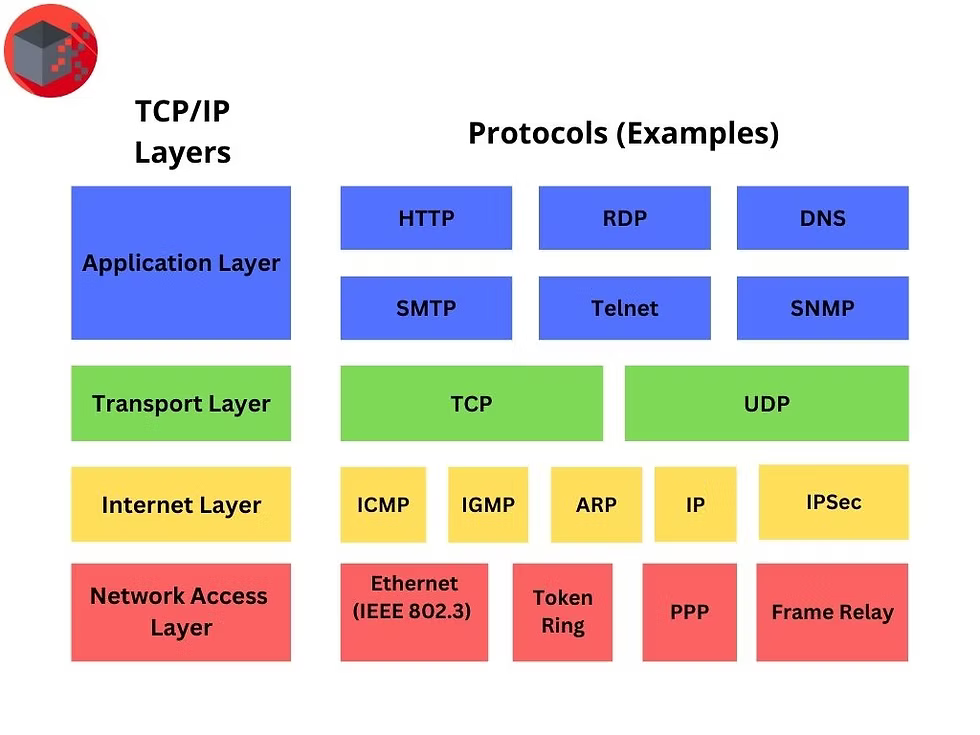
\includegraphics[width=0.5\linewidth]{Figures/tcp_ip_model.png}
    \caption{Kiến trúc 4 tầng của mô hình TCP/IP}
\end{figure}

\textbf{Mô hình TCP/IP gồm 4 tầng:}

\begin{enumerate}
    \item \textbf{Tầng giao diện mạng (Network Interface Layer):}  
    Còn gọi là tầng liên kết hoặc tầng truy cập mạng. Chịu trách nhiệm truyền và nhận dữ liệu qua phương tiện truyền dẫn vật lý. Tầng này tương đương với tầng Vật lý và tầng Liên kết dữ liệu trong mô hình OSI.

    \item \textbf{Tầng Internet (Internet Layer):}  
    Đảm nhiệm việc định tuyến và định địa chỉ cho các gói dữ liệu giữa các mạng. Giao thức chính tại tầng này là IP (Internet Protocol), cùng với các giao thức phụ trợ như ICMP (Internet Control Message Protocol), ARP (Address Resolution Protocol).

    \item \textbf{Tầng giao vận (Transport Layer):}  
    Cung cấp cơ chế truyền dữ liệu giữa các tiến trình ứng dụng trên các máy tính khác nhau. Hai giao thức chính là:
    \begin{itemize}
        \item TCP (Transmission Control Protocol): Truyền dữ liệu đáng tin cậy, đảm bảo thứ tự và kiểm soát lỗi.
        \item UDP (User Datagram Protocol): Truyền dữ liệu không đảm bảo, tốc độ cao, dùng trong các ứng dụng thời gian thực.
    \end{itemize}

    \item \textbf{Tầng ứng dụng (Application Layer):}  
    Cung cấp giao diện trực tiếp với người dùng hoặc chương trình ứng dụng. Bao gồm các giao thức như: HTTP (truy cập web), FTP (truyền tệp), SMTP (gửi email), DNS (phân giải tên miền)…

\end{enumerate}

\textbf{So sánh với mô hình OSI:}

\begin{table}[H]
    \centering
    \caption{So sánh mô hình OSI và TCP/IP}
    \begin{tabular}{|c|c|}
        \hline
        \textbf{Mô hình OSI} & \textbf{Mô hình TCP/IP} \\
        \hline
        7. Application         & Application \\
        6. Presentation        & \\
        5. Session             & \\
        \hline
        4. Transport           & Transport \\
        \hline
        3. Network             & Internet \\
        \hline
        2. Data Link           & Network Interface \\
        1. Physical            & \\
        \hline
    \end{tabular}
\end{table}

Mô hình TCP/IP đơn giản hơn OSI và được áp dụng rộng rãi trong thực tế. Sự phân tầng rõ ràng của nó giúp việc triển khai, chuẩn hóa và khắc phục lỗi trong hệ thống mạng trở nên hiệu quả hơn.

\subsubsection{Giao thức TCP}

TCP\cite{rfc9293} (Transmission Control Protocol) là một giao thức lớp giao vận trong bộ giao thức TCP/IP, được thiết kế để cung cấp dịch vụ truyền dữ liệu tin cậy giữa các thiết bị đầu cuối trong mạng. Khác với UDP, TCP đảm bảo rằng dữ liệu đến đúng thứ tự, không bị mất mát, trùng lặp hoặc hư hỏng thông qua các cơ chế kiểm soát lỗi và điều khiển luồng.

\textbf{Đặc điểm chính của TCP:}
\begin{itemize}
    \item \textbf{Kết nối hướng phiên (connection-oriented):} Trước khi truyền dữ liệu, TCP thiết lập kết nối giữa hai thiết bị bằng quy trình bắt tay ba bước (three-way handshake).
    \item \textbf{Truyền dữ liệu đáng tin cậy:} TCP sử dụng cơ chế xác nhận (ACK), đánh số thứ tự gói tin (sequence number), kiểm tra lỗi (checksum) để đảm bảo dữ liệu truyền đến đúng đích và đúng thứ tự.
    \item \textbf{Kiểm soát luồng (flow control):} Điều chỉnh tốc độ truyền dữ liệu giữa hai thiết bị nhằm tránh hiện tượng nghẽn hoặc tràn bộ đệm.
    \item \textbf{Điều khiển tắc nghẽn (congestion control):} Giảm lưu lượng khi mạng bị quá tải, sử dụng các thuật toán như Slow Start, Congestion Avoidance, Fast Retransmit và Fast Recovery.
\end{itemize}

\textbf{Quy trình bắt tay ba bước (Three-way Handshake, hình \ref{fig:tcp_handshake} ):}
\begin{enumerate}
    \item Client gửi một gói tin SYN đến Server để yêu cầu kết nối.
    \item Server phản hồi bằng gói tin SYN-ACK để đồng ý kết nối.
    \item Client gửi gói tin ACK để xác nhận, sau đó kết nối được thiết lập.
\end{enumerate}

\begin{figure}[!ht]
    \centering
    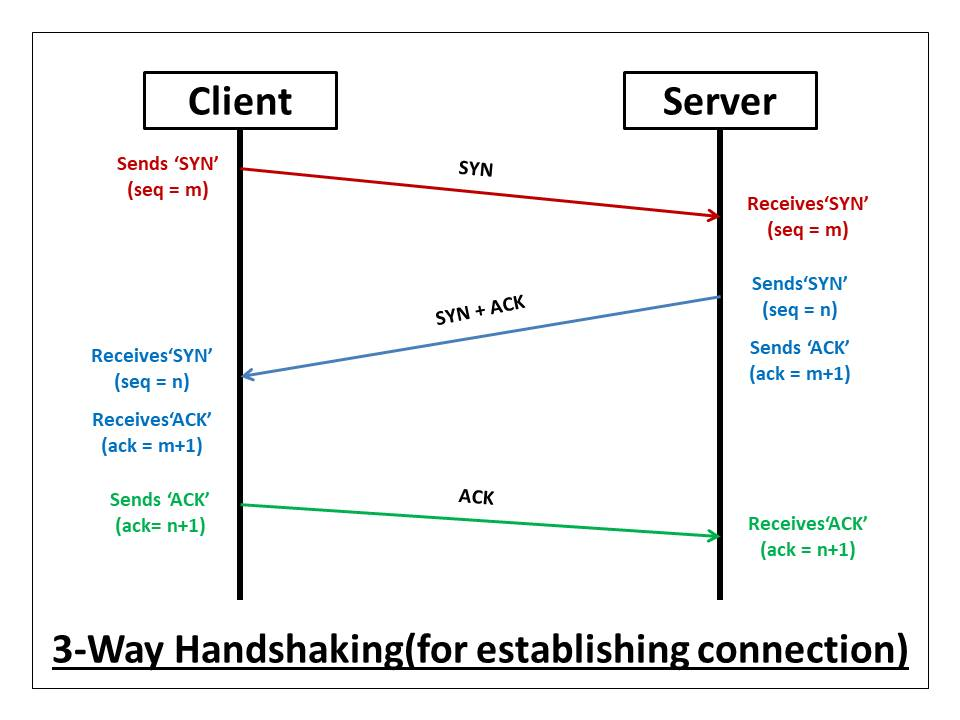
\includegraphics[width=0.6\linewidth]{Figures/tcp_handshake.jpg}
    \caption{Quy trình bắt tay ba bước trong TCP}
    \label{fig:tcp_handshake}
\end{figure}

\textbf{Cấu trúc gói tin TCP (hình \ref{fig:TCP-packet-format })}

\begin{figure}[!ht]
    \centering
    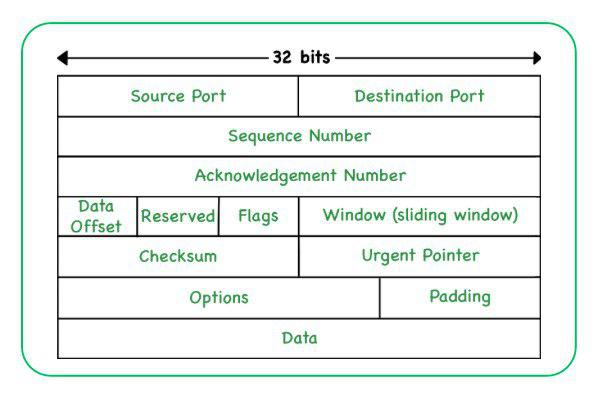
\includegraphics[width=0.6\linewidth]{Figures/TCP-packet-format.jpg}
    \caption{Cấu trúc gói tin TCP}
    \label{fig:TCP-packet-format }
\end{figure}

\begin{itemize}
    \item \textbf{Port nguồn / Port đích:} Xác định ứng dụng gửi và nhận.
    \item \textbf{Sequence Number:} Đánh dấu thứ tự byte trong dòng dữ liệu.
    \item \textbf{Acknowledgment Number:} Xác nhận đã nhận đến byte nào.
    \item \textbf{Flags:} Các cờ điều khiển như SYN, ACK, FIN...
    \item \textbf{Checksum:} Kiểm tra lỗi dữ liệu.
\end{itemize}

\textbf{Ứng dụng của TCP:}  
TCP được sử dụng trong các ứng dụng yêu cầu độ tin cậy cao như: trình duyệt web (HTTP/HTTPS), gửi email (SMTP, IMAP), truyền file (FTP), truy cập từ xa (SSH, Telnet)...

TCP tuy có độ trễ cao hơn UDP nhưng đổi lại cung cấp một kênh truyền thông ổn định, đáng tin cậy, phù hợp với hầu hết các ứng dụng Internet phổ biến.

\FloatBarrier
\subsubsection{Giao thức UDP}

UDP\cite{rfc768} (User Datagram Protocol) là một giao thức ở tầng giao vận trong bộ giao thức TCP/IP, cung cấp phương thức truyền dữ liệu đơn giản, không kết nối (connectionless) và không đảm bảo độ tin cậy. UDP được sử dụng trong các ứng dụng yêu cầu tốc độ cao, truyền dữ liệu thời gian thực hoặc có cơ chế kiểm soát lỗi riêng tại tầng ứng dụng.

\textbf{Đặc điểm chính của UDP:}
\begin{itemize}
    \item \textbf{Không kết nối (Connectionless):} Không cần thiết lập phiên giao tiếp trước khi gửi dữ liệu, mỗi gói tin được truyền độc lập.
    \item \textbf{Không đảm bảo độ tin cậy:} UDP không có cơ chế xác nhận (ACK), đánh số thứ tự hay truyền lại gói bị mất.
    \item \textbf{Không kiểm soát luồng hay tắc nghẽn:} Việc kiểm soát được giao cho tầng ứng dụng nếu cần.
    \item \textbf{Hiệu năng cao:} Do không có overhead kiểm soát phức tạp, UDP có độ trễ thấp và tốc độ truyền nhanh hơn TCP.
\end{itemize}

\textbf{Cấu trúc gói tin UDP:}

\begin{figure}[H]
    \centering
    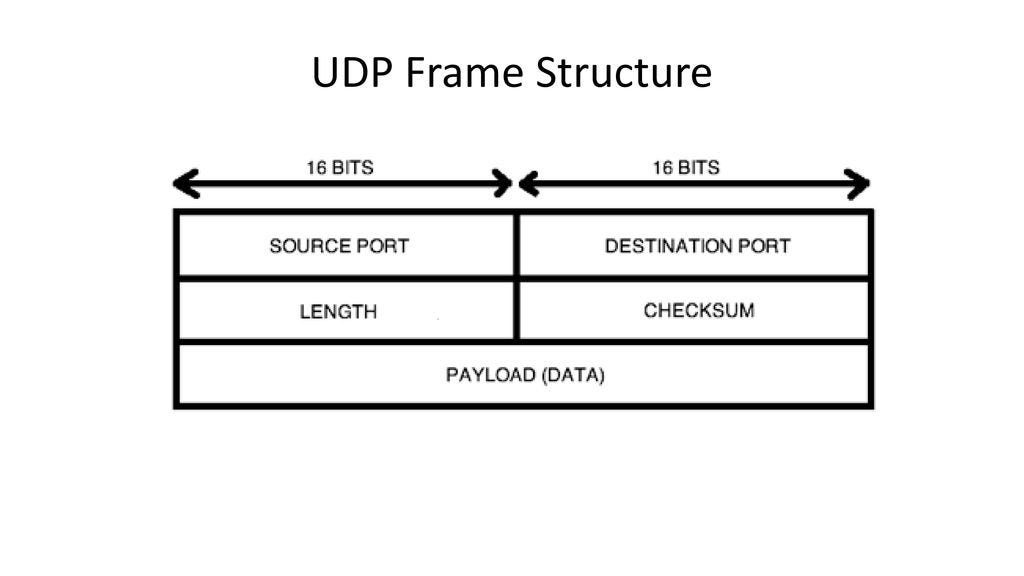
\includegraphics[width=0.8\linewidth]{Figures/udp-packet format.jpg}
    \caption{Cấu trúc gói tin UDP}
    \label{fig:udp-packet format}
\end{figure}


\begin{itemize}
    \item \textbf{Port nguồn (Source Port):} Xác định ứng dụng gửi.
    \item \textbf{Port đích (Destination Port):} Xác định ứng dụng nhận.
    \item \textbf{Độ dài (Length):} Tổng chiều dài của gói UDP (header + dữ liệu).
    \item \textbf{Checksum:} Kiểm tra lỗi cho phần header và dữ liệu.
\end{itemize}


\textbf{Ưu điểm của UDP:}
\begin{itemize}
    \item Tốc độ truyền nhanh, độ trễ thấp.
    \item Phù hợp với các ứng dụng thời gian thực (real-time) như VoIP, video streaming, game online...
    \item Dễ dàng broadcast hoặc multicast dữ liệu đến nhiều thiết bị.
\end{itemize}

\textbf{Hạn chế của UDP:}
\begin{itemize}
    \item Không đảm bảo dữ liệu được nhận hoặc nhận đúng thứ tự.
    \item Không có cơ chế tự động phát hiện và truyền lại khi mất gói.
\end{itemize}

\textbf{Ứng dụng của UDP:}
UDP được sử dụng trong các ứng dụng như: DNS, DHCP, TFTP, truyền video/audio trực tiếp, gọi điện qua mạng (VoIP), hoặc các giao thức mạng yêu cầu gửi nhanh, không cần xác nhận.

Mặc dù không đảm bảo độ tin cậy như TCP, nhưng UDP là lựa chọn tối ưu cho các tình huống cần ưu tiên tốc độ và độ trễ thấp hơn là tính chính xác tuyệt đối.

\subsection{Các công nghệ liên quan}

\subsubsection{Vi điều khiển STM32}

STM32\cite{st_rm_f4} là dòng vi điều khiển 32-bit do hãng STMicroelectronics phát triển, dựa trên kiến trúc ARM Cortex-M. Dòng STM32 rất phổ biến trong các ứng dụng nhúng (embedded systems) nhờ vào hiệu năng cao, mức tiêu thụ điện năng thấp, tích hợp nhiều ngoại vi và hỗ trợ phần mềm mạnh mẽ.

\textbf{Các đặc điểm nổi bật của STM32:}
\begin{itemize}
    \item \textbf{Kiến trúc ARM Cortex-M:} STM32 sử dụng các lõi ARM như Cortex-M0, M3, M4 và M7 tùy theo dòng sản phẩm, cho phép cân bằng giữa hiệu năng và tiêu thụ điện năng.
    
    \item \textbf{Tốc độ xử lý cao:} Tốc độ xung nhịp từ 32 MHz đến hơn 400 MHz, hỗ trợ thực hiện các tác vụ thời gian thực và xử lý tín hiệu.

    \item \textbf{Tích hợp nhiều ngoại vi:} Bao gồm GPIO, UART, SPI, I2C, CAN, USB, ADC, DAC, PWM... hỗ trợ kết nối với nhiều loại cảm biến và thiết bị ngoại vi.

    \item \textbf{Đa dạng dòng sản phẩm:} STM32 được chia thành nhiều dòng như STM32F0, F1, F3, F4, F7, H7… phù hợp với nhiều mức độ ứng dụng từ đơn giản đến cao cấp.

    \item \textbf{Công cụ hỗ trợ phát triển mạnh mẽ:} Hỗ trợ nhiều IDE như STM32CubeIDE, Keil, IAR và thư viện phần mềm STM32Cube HAL, LL. Ngoài ra còn có công cụ cấu hình ngoại vi STM32CubeMX rất thuận tiện cho việc thiết lập ban đầu.
\end{itemize}

\FloatBarrier
\textbf{Ứng dụng của STM32:}
STM32 được sử dụng rộng rãi trong các lĩnh vực:
\begin{itemize}
    \item Thiết bị IoT và điều khiển từ xa.
    \item Thiết bị đo lường và điều khiển công nghiệp.
    \item Thiết bị y tế, robot, và hệ thống nhúng trong ô tô.
    \item Thiết bị tiêu dùng như đồng hồ thông minh, máy chơi game, thiết bị điều khiển ánh sáng và âm thanh.
\end{itemize}

\begin{figure}[!ht]
    \centering
    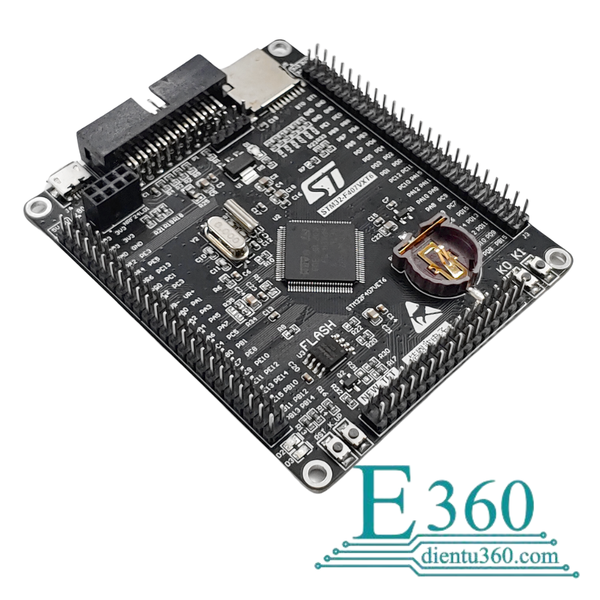
\includegraphics[width=0.4\linewidth]{Figures/stm32f407vet6-dev-kit.png}
    \caption{KIT phát triển STM32F407VET6 ARM Cortex-M4}
    \label{fig:stm32f407vet6-dev-kit}
\end{figure}

STM32 là một nền tảng lý tưởng cho các ứng dụng nhúng nhờ khả năng mở rộng, độ ổn định cao và tài nguyên phát triển phong phú. Việc nắm vững STM32 giúp rút ngắn thời gian phát triển và tăng tính hiệu quả trong các dự án điện tử.

\subsubsection{Ngôn ngữ lập trình C/C++}

Ngôn ngữ lập trình C và C++ là hai ngôn ngữ phổ biến trong phát triển hệ thống nhúng và lập trình điều khiển phần cứng. Chúng cung cấp khả năng kiểm soát trực tiếp bộ nhớ, hiệu năng cao và tương thích tốt với các tài nguyên phần cứng, điều này làm cho chúng trở thành lựa chọn hàng đầu trong các ứng dụng thời gian thực như lập trình vi điều khiển STM32.

\textbf{Ngôn ngữ C}
\begin{itemize}
    \item Là ngôn ngữ lập trình thủ tục, đơn giản, dễ hiểu, và rất phù hợp với việc lập trình cấp thấp.
    \item Cho phép truy cập trực tiếp đến bộ nhớ thông qua con trỏ.
    \item Có thư viện chuẩn nhỏ gọn, dễ tích hợp vào hệ thống không có hệ điều hành.
    \item Là ngôn ngữ chính được sử dụng trong các trình biên dịch và thư viện hỗ trợ cho STM32 như STM32Cube HAL, CMSIS.
\end{itemize}

\textbf{Ngôn ngữ C++}
\begin{itemize}
    \item Là phần mở rộng của C, hỗ trợ lập trình hướng đối tượng, giúp tổ chức mã nguồn tốt hơn, dễ bảo trì và mở rộng.
    \item Cung cấp tính năng kế thừa, đa hình và đóng gói, rất hữu ích trong phát triển phần mềm phức tạp hoặc quy mô lớn.
    \item Cho phép sử dụng các cấu trúc hiện đại như class, template, STL (Standard Template Library).
    \item Ngày càng được sử dụng trong lập trình nhúng hiện đại, đặc biệt khi kết hợp với hệ điều hành thời gian thực (RTOS).
\end{itemize}

\textbf{Ưu điểm khi dùng C/C++ trong lập trình vi điều khiển:}
\begin{itemize}
    \item Hiệu năng cao, thời gian thực.
    \item Có thể tối ưu kích thước mã nguồn và bộ nhớ sử dụng.
    \item Dễ dàng tích hợp với trình biên dịch như GCC, Keil, IAR...
    \item Được hỗ trợ rộng rãi trong cộng đồng và các tài liệu kỹ thuật.
\end{itemize}

\textbf{Ứng dụng:}  
C/C++ là công cụ chính để lập trình firmware cho vi điều khiển, viết driver điều khiển phần cứng, giao tiếp với cảm biến, mô-đun truyền thông (UART, SPI, I2C), và xây dựng các hệ thống điều khiển tự động.

\subsubsection{Môi trường phát triển phần mềm NodeJS}

Node.js\cite{nodejs_docs} là một môi trường chạy mã JavaScript phía máy chủ, được xây dựng trên nền tảng V8 JavaScript Engine của Google. Không giống như JavaScript truyền thống vốn chỉ chạy trên trình duyệt, Node.js cho phép thực thi mã JavaScript trong môi trường máy chủ (server-side), hỗ trợ xây dựng các ứng dụng mạng có hiệu năng cao như web server, API, công cụ dòng lệnh và hệ thống xử lý thời gian thực.

\textbf{Đặc điểm nổi bật của Node.js:}
\begin{itemize}
    \item \textbf{Mô hình xử lý bất đồng bộ (asynchronous) và không chặn (non-blocking):} Node.js sử dụng vòng lặp sự kiện (event loop) và callback để xử lý nhiều yêu cầu đồng thời mà không bị treo luồng chính.
    
    \item \textbf{Một luồng (single-threaded) nhưng hiệu quả:} Thay vì tạo nhiều luồng như các nền tảng truyền thống, Node.js hoạt động hiệu quả bằng cách sử dụng cơ chế I/O bất đồng bộ để phục vụ nhiều yêu cầu cùng lúc.

    \item \textbf{Quản lý gói mạnh mẽ với NPM (Node Package Manager):} NPM là hệ sinh thái thư viện mã nguồn mở lớn nhất thế giới, hỗ trợ hàng triệu gói phần mềm để tích hợp vào dự án Node.js.

    \item \textbf{Tương thích tốt với JSON và REST API:} Node.js phù hợp để xây dựng các ứng dụng backend hiện đại kết hợp với cơ sở dữ liệu NoSQL (như MongoDB) hoặc SQL.

    \item \textbf{Khả năng mở rộng tốt:} Có thể mở rộng theo chiều ngang (scale-out) dễ dàng bằng cách tạo nhiều tiến trình (cluster) và phân phối tải.
\end{itemize}

\textbf{Ứng dụng của Node.js:}
\begin{itemize}
    \item Xây dựng Web server và API RESTful.
    \item Hệ thống giám sát, điều khiển thiết bị IoT.
    \item Ứng dụng thời gian thực như chat, truyền phát dữ liệu (WebSocket).
    \item Các công cụ tự động hóa (build tool, CLI).
\end{itemize}

\textbf{Công cụ hỗ trợ phát triển:}
\begin{itemize}
    \item \textbf{Visual Studio Code (VSCode):} IDE phổ biến hỗ trợ đầy đủ Node.js.
    \item \textbf{Express.js:} Framework web phổ biến trên nền Node.js.
    \item \textbf{Nodemon:} Tự động khởi động lại server khi có thay đổi mã nguồn.
    \item \textbf{Debug và profiling:} Hỗ trợ bởi Chrome DevTools, VSCode, hoặc các công cụ như `node --inspect`.
\end{itemize}

Node.js là một công nghệ lý tưởng cho các ứng dụng hiện đại yêu cầu khả năng xử lý nhiều kết nối đồng thời, phản hồi nhanh và dễ triển khai. Với cộng đồng lớn và tài nguyên phong phú, Node.js ngày càng được sử dụng rộng rãi trong phát triển phần mềm, đặc biệt là trong các hệ thống phân tán và IoT.

\FloatBarrier
\subsection{Lựa chọn công nghệ phù hợp}


\subsubsection{Chip Ethernet để kết nối với mạng LAN}

Yêu cầu đặt ra là lựa chọn chip có thể kết nối Ethernet để thiết bị đọc ghi màn hình xăng dầu có thể tham gia mạng LAN, từ đó kết nối và gửi dữ liệu cho phần mềm giải mã.

Chip Ethernet cần đáp ứng nhu cầu sau:

\begin{itemize}
    \item Giao tiếp với vi điều khiển trung tâm qua SPI do SPI có tốc độ truyền cao, có thể truyền dữ liệu liên tục không ngắt quãng.
    \item Hỗ trợ sẵn các giao thức: IPv4, TCP, UDP.
    \item Phổ biến và giá thành vừa phải.
    \item Ưu tiên chip có sẵn thư viện hỗ trợ bằng ngôn ngữ C/C++
\end{itemize}


\begin{longtable}{|>{\raggedright\arraybackslash}p{1.5cm}|>{\raggedright\arraybackslash}p{2.7cm}|>{\raggedright\arraybackslash}p{2.7cm}|>{\raggedright\arraybackslash}p{2.7cm}|>{\raggedright\arraybackslash}p{2.7cm}|}

\caption{So sánh các chip Ethernet phổ biến} \\
\hline
\textbf{Tiêu chí} & \textbf{W5500}\cite{wiznet_w5500} & \textbf{ENC28J60}\cite{ENC28J60_Data_Sheet} & \textbf{W5100S}\cite{wiznet_W5100S} & \textbf{LAN8720A\cite{LAN8720A_Data_Sheet}} \\
\hline
\endfirsthead

\hline
\textbf{Tiêu chí} & \textbf{W5500} & \textbf{ENC28J60} & \textbf{W5100S} & \textbf{LAN8720A} \\
\hline
\endhead

\hline
\endfoot

\hline
\endlastfoot

\textbf{Giao tiếp với vi điều khiển} & 
SPI tốc độ cao (80 MHz), 8 sockets & 
SPI (tối đa 20MHz, phụ thuộc MCU xử lý nhiều) & 
SPI (nhanh và đơn giản, 70MHz), 4 sockets & 
RMII (cần vi điều khiển có MAC tích hợp) \\
\hline

\textbf{Hỗ trợ giao thức mạng} & 
Tích hợp phần cứng: IPv4, TCP, UDP & 
Chỉ Ethernet layer (TCP/IP xử lý bằng phần mềm) & 
Tích hợp IPv4, TCP, UDP & 
Không tích hợp TCP/IP stack, chỉ là PHY \\
\hline

\textbf{Tốc độ truyền dữ liệu} & 
SPI 80 MHz, hiệu năng ổn định & 
SPI 25 MHz (10 Mbps), hiệu năng thấp  & 
SPI 70 MHz, cải tiến từ W5100 & 
10/100 Mbps (phụ thuộc MAC của MCU) \\ 
\hline

\textbf{Tài liệu và thư viện hỗ trợ} & 
Rất phổ biến, Có thư viện ngôn ngữ C & 
Có thư viện C & 
Thư viện tương tự W5500, hỗ trợ tốt & 
Cần tích hợp LWIP hoặc stack riêng của MCU \\
\hline

\textbf{Độ phổ biến} & 
Phổ biến trong hệ thống nhúng hiện đại & 
Phổ biến trong hệ thống giá rẻ hoặc cũ & 
Ít phổ biến hơn W5500 nhưng cùng họ Wiznet & 
Thường dùng với vi điều khiển có MAC riêng (ESP32, STM32F4+) \\
\hline

\textbf{Giá thành (tham khảo)} & 
~\$3.67 & 
~\$4.00 & 
\$3.2 - \$3.5 & 
~\$1.03 \\
\hline

\end{longtable}

Từ bảng liệt kê trên, chọn chip \textbf{W5500} là chip Ethernet cho mạch phần cứng Thiết bị đọc ghi màn hình cây xăng.

\begin{figure}[!ht]
    \centering
    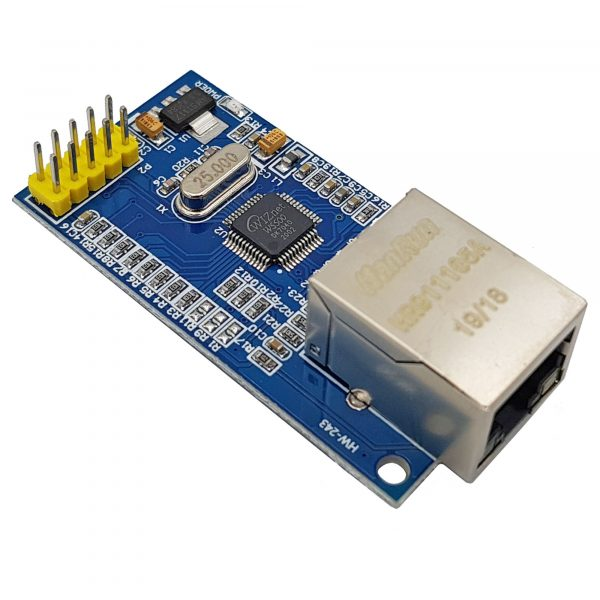
\includegraphics[width=0.8\linewidth]{Figures/module-ethernet-w5500.jpg}
    \caption{Module Ethernet W5500}
    \label{fig:}
\end{figure}
\FloatBarrier

\subsubsection{Vi điều khiển trung tâm cho thiết bị đọc màn hình}

Yêu cầu lựa chọn:
\begin{itemize}
    \item Có 2 cổng giao tiếp SPI: mục đích để giao tiếp với khối chuyển đổi tín hiệu và với khối Ethernet. 
    \item Bộ nhớ flash lớn hơn 220KB (chứa được 2 firmware, mỗi firm ~ 110kB)
    \item Nhanh và ổn định, dễ dàng mở rộng
\end{itemize}

Từ những yêu cầu trên , lựa chọn \textbf{STM32F407VET6} là vi điều khiển xử lý trung tâm. Các tính năng nổi bật của STM32F407VET6:

\begin{itemize}
    \item Vi điều khiển sử dụng lõi ARM Cortex-M4 32-bit, tốc độ tối đa 168 MHz, tích hợp bộ xử lý dấu chấm động (FPU) và tập lệnh DSP, phù hợp cho các ứng dụng điều khiển và xử lý tín hiệu thời gian thực.
    
    \item Bộ nhớ Flash Main Memory 512 KB, được chia thành các sector như sau:  
    
    \begin{itemize}
        \item Sector 0-3: mỗi sector 16 KB  
        \item Sector 4: 64 KB  
        \item Sector 5, 6 và 11: mỗi sector 128-KB  
    \end{itemize}

    \item Cho phép linh hoạt khi lưu nhiều firmware (ví dụ dual-bank firmware upgrade), hoặc phân vùng cho bootloader, data log, cấu hình...

    \item Tích hợp 3 cổng SPI (SPI1, SPI2, SPI3), hỗ trợ chế độ master/slave, tốc độ tối đa đến 42 MHz (SPI1) và 21 MHz (SPI2/SPI3). Phù hợp cho các giao tiếp tốc độ cao như ADC ngoại vi và module Ethernet SPI.

    \item Có tổng cộng 17 bộ Timer, gồm 12 timer 16-bit và 2 timer 32-bit. Hỗ trợ nhiều chế độ: PWM, encoder, input capture, output compare, rất hữu ích trong điều khiển động cơ, đo thời gian hoặc phát xung.

    \item Hỗ trợ nhiều chuẩn giao tiếp ngoại vi: UART, I2C, USB OTG, CAN, SDIO, Ethernet MAC - thuận tiện cho mở rộng và kết nối các module chức năng khác.

    \item Hoạt động với điện áp 1.8 V đến 3.6 V, hỗ trợ các chế độ tiết kiệm năng lượng như Sleep, Stop, và Standby - phù hợp cho ứng dụng nhúng có yêu cầu tiêu thụ điện thấp.
\end{itemize}

\subsection{Kết luận chương} Chương này đã đưa ra những nền tảng lý thuyết chính để thiết kế thiết bị đọc ghi màn hình cột bơm xăng dầu. Đồng thời cũng đưa ra so sánh và lựa chọn linh kiện phù hợp cho 2 khối quan trọng là vi điều khiển trung tâm (STM32F407VET6) và chip giao tiếp Ethernet (W5500), làm cơ sở cho quá trình thiết kế chi tiết mạch cứng và phần mềm, sẽ được trình bày ở Chương 3.
